\section{Conversion and the Appearance of the Input}
\label{app:details}
\label{app:appearance}

\begin{figure*}[!t]
\centering
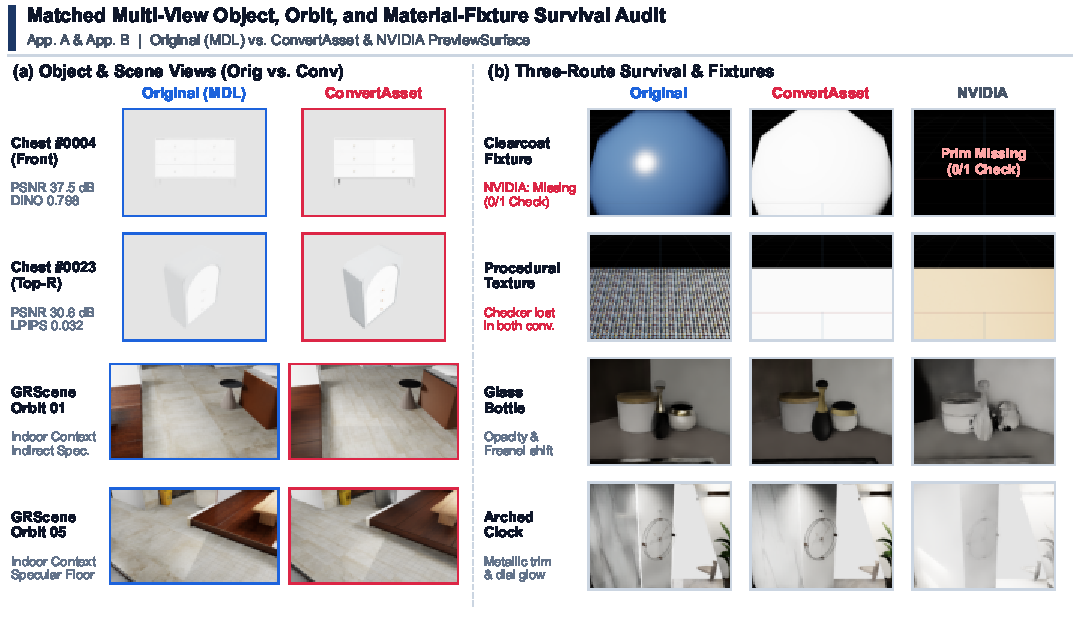
\includegraphics[width=\textwidth]{app_fig1_appearance_and_materials.pdf}
\caption{\textbf{Controlled multi-view appearance metrics and three-route material fixture survival.}
\emph{(a)} Representative paired renders between native \textsc{NVIDIA MDL} (\original{}) and lowered \usdps{} (\converted{}) across four-asset multi-view chest-of-drawers renders (reported quantitatively in Table~\ref{tab:app-proxy}) and \textsc{GRScenes} scene orbits preserving room context and indirect reflections.
\emph{(b)} Side-by-side survival comparison across \original{}, \textsc{ConvertAsset}, and the \textsc{NVIDIA} preview conversion baseline covering diagnostic fixtures (clearcoat and procedural checker) and paired \textsc{GRScenes} targets (Section~\ref{app:materials} and Table~\ref{tab:app-materials}).}
\label{fig:app-appearance-materials}
\end{figure*}

Material translation alters surface shading networks while preserving scene meshes, object transforms, camera parameters, and lighting placement. In particular, \textsc{ConvertAsset} recursively traverses \textsc{USD} references, payloads, sublayers, and variant sets, writing sibling converted layers whose bindings target \usdps{} counterparts while leaving the source \textsc{MDL} scenes unmodified. Base color, roughness, metallic response, normal maps, and texture connections are mapped explicitly, whereas higher-order clearcoat, transmission, and procedural shaders require coarse approximations (detailed further in~\ref{app:materials}).

\subsection{Matched multi-view object appearance}
To isolate multi-view perceptual fidelity prior to indoor scene evaluation, four chest-of-drawers assets from a preliminary toolkit benchmark \citep{Zhu2026Evaluating} are each rendered from six canonical camera angles (front, back, left, right, and two elevated front views), yielding 24 paired renders (Table~\ref{tab:app-proxy}). Pixel error uses $\mathrm{PSNR} = 10\log_{10}(1/\mathrm{MSE})$ on $[0,1]$-scaled RGB frames; structural similarity uses $\mathrm{SSIM}$ \citep{Wang2004Image}; perceptual distance uses \textsc{VGG}-backbone $\mathrm{LPIPS}$ \citep{Zhang2018Unreasonable}; and semantic feature cosine similarity $f(I^O)^\top f(I^C)/(\|f(I^O)\|_2\|f(I^C)\|_2)$ uses \textsc{CLIP} ViT-B/32 \citep{Radford2021Learning} and \textsc{DINOv2} \citep{Oquab2023DINOv2}.

\begin{table}[!htbp]
\centering\small
\resizebox{\linewidth}{!}{% Generated by appendix/build_tables.py; source hashes in table_sources.json.
\begin{tabular}{lrrrrrr}
\toprule
Asset & Pairs & PSNR & SSIM & LPIPS & CLIP & DINOv2 \\
\midrule
Chest 0004 & 6 & 37.51 & 0.991 & 0.019 & 0.921 & 0.798 \\
Chest 0011 & 6 & 36.30 & 0.993 & 0.017 & 0.956 & 0.922 \\
Chest 0023 & 6 & 30.59 & 0.986 & 0.032 & 0.938 & 0.905 \\
Chest 0029 & 6 & 37.68 & 0.991 & 0.014 & 0.885 & 0.864 \\
All & 24 & 35.52 & 0.990 & 0.020 & 0.925 & 0.872 \\
\bottomrule
\end{tabular}
}
\caption{Matched object renders averaged over six camera directions per asset. Higher PSNR (dB), SSIM, CLIP, and DINOv2 indicate stronger visual similarity; lower LPIPS indicates closer perceptual match.}
\label{tab:app-proxy}
\end{table}

Aggregate fidelity across all 24 views is high ($\mathrm{PSNR}=35.52\,\mathrm{dB}$, $\mathrm{SSIM}=0.990$, $\mathrm{LPIPS}=0.020$), yet per-asset profiles diverge meaningfully: Chest~0023 records the lowest PSNR ($30.59\,\mathrm{dB}$) and highest LPIPS ($0.032$), whereas Chest~0004 records the lowest DINOv2 similarity ($0.798$) despite high PSNR ($37.51\,\mathrm{dB}$). Figure~\ref{fig:app-appearance-materials}(a) places the chest views alongside indoor \textsc{GRScenes} camera orbits, illustrating why holistic object metrics still allow localized changes in specular reflections, wood sheen, and nearby surface lighting.
